\documentclass{standalone}
\usepackage{tikz}
\usetikzlibrary{positioning, decorations.pathreplacing}

\begin{document}

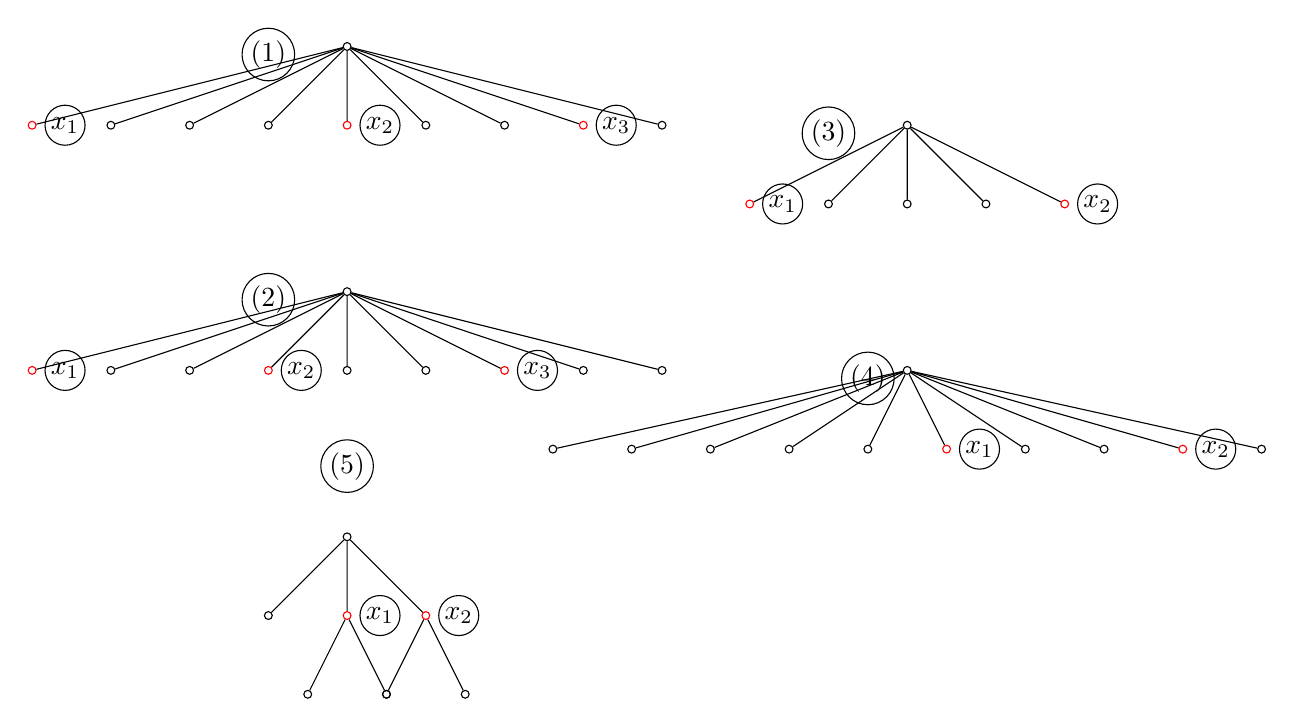
\begin{tikzpicture}[every node/.style={circle, draw, inner sep=1pt},
  level distance=1cm, sibling distance=1cm]

% Tree (1)
\node (1-1) {} 
    child {node[red] (1-2) {}}
    child {node (1-3) {}}
    child {node (1-4) {}}
    child {node (1-5) {}}
    child {node[red] (1-6) {}}
    child {node (1-7) {}}
    child {node (1-8) {}}
    child {node[red] (1-9) {}}
    child {node (1-10) {}};

\node[above=0.5cm of 1-5] {(1)};

% Tree (2)
\node[below=3cm of 1-1] (2-1) {}
    child {node[red] (2-2) {}}
    child {node (2-3) {}}
    child {node (2-4) {}}
    child {node[red] (2-5) {}}
    child {node (2-6) {}}
    child {node (2-7) {}}
    child {node[red] (2-8) {}}
    child {node (2-9) {}}
    child {node (2-10) {}};

\node[above=0.5cm of 2-5] {(2)};

% Tree (3)
\node[right=3cm of 1-10] (3-1) {}
    child {node[red] (3-2) {}}
    child {node (3-3) {}}
    child {node (3-4) {}}
    child {node (3-5) {}}
    child {node[red] (3-6) {}};

\node[above=0.5cm of 3-3] {(3)};

% Tree (4)
\node[below=3cm of 3-1] (4-1) {}
    child {node (4-2) {}}
    child {node (4-3) {}}
    child {node (4-4) {}}
    child {node (4-5) {}}
    child {node (4-6) {}}
    child {node[red] (4-7) {}}
    child {node (4-8) {}}
    child {node (4-9) {}}
    child {node[red] (4-10) {}}
    child {node (4-11) {}};

\node[above=0.5cm of 4-6] {(4)};

% Tree (5)
\node[below=3cm of 2-1] (5-1) {}
    child {node (5-2) {}}
    child {node[red] (5-3) {}
        child {node (5-4) {}}
        child {node (5-5) {}}
    }
    child {node[red] (5-6) {}
        child {node (5-7) {}}
        child {node (5-8) {}}
    };

\node[above=0.5cm of 5-1] {(5)};

% Labels
\node[right=0.1cm of 1-2] {$x_1$};
\node[right=0.1cm of 1-6] {$x_2$};
\node[right=0.1cm of 1-9] {$x_3$};

\node[right=0.1cm of 2-2] {$x_1$};
\node[right=0.1cm of 2-5] {$x_2$};
\node[right=0.1cm of 2-8] {$x_3$};

\node[right=0.1cm of 3-2] {$x_1$};
\node[right=0.1cm of 3-6] {$x_2$};

\node[right=0.1cm of 4-7] {$x_1$};
\node[right=0.1cm of 4-10] {$x_2$};

\node[right=0.1cm of 5-3] {$x_1$};
\node[right=0.1cm of 5-6] {$x_2$};

\end{tikzpicture}

\end{document}